\documentclass[a4paper,12pt,twoside]{article}%方框内设置默认的正文字体大小
%基于北京航空航天大学仪器科学与光电工程学院实验报告及课程报告排版得来,类似于毕业论文排版格式
%后续将更新毕业论文排版格式
\usepackage{graphicx,float}%使用图的宏包,使用图的浮动体宏包,引入参数H使图像紧跟当前文字
\usepackage{caption} %使用图表标题的宏包
\usepackage[colorlinks=true,pdfstartview=FitH,%
linkcolor=black,anchorcolor=violet,citecolor=magenta]{hyperref}%加载hyperref宏包,使用超链接
\usepackage{setspace}%用于设置行间距列间距等命令的宏包
\usepackage{array}%设置列表高度宽度的宏包
\usepackage{zhnumber}%使用中文数字编号的宏包
\usepackage{titlesec,titletoc}%使用标题自定义形式的宏包和使用目录自定义形式的宏包
\usepackage{siunitx}%物理学单位宏包
\usepackage{tabularx}%让表格宽度等于页面宽度
\usepackage{makecell}%单个表格单元调整的宏包
\usepackage{subfigure} %%使用子图的宏包
\usepackage[backend=biber,bibstyle=gb7714-2015,%nature,%%加载biblatex宏包,使用参考文献
citestyle=gb7714-2015%,backref=true%%其中后端backend使用biber
,url=false,doi=false
]{biblatex}%标注(引用)样式citestyle,著录样式bibstyle都采用gb7714-2015样式
% \usepackage{pgfplots}%类似tikz的一个画图库,主要画统计图
\usepackage{../customStyle}
% \usepackage[lite,subscriptcorrection,slantedGreek,nofontinfo]{mtpro2}%使用mathtimepro2商业字体作为数学环境,并不推荐

%biblatex宏包的参考文献数据源加载方式,注意book.bib应当与.tex文件在同一目录下,不然有可能会报错
\addbibresource[location=local]{book.bib}
%%% 下面的命令重定义页面边距,使其符合中文刊物习惯 %%%%
\setlength{\oddsidemargin}{0.63cm}  % 3.17cm - 1 inch
\setlength{\evensidemargin}{\oddsidemargin}
% 重定义页眉
% \pagestyle{beihang}
% \fancyhead[CO]{机电仿真实验报告}%

\graphicspath{{./fig}}

\begin{document}
{
  %% ----------- 封面部分 ------------ %%
\pagestyle{empty}
\begin{figure}
  
\includegraphics{title.jpg}
\end{figure}
\begin{center}

  \begin{figure}[h]

    \centering
    
\includegraphics[]{title.png}\par
    \vspace{4em}
    \large{\chuhao\heiti{机电仿真实验}}\par
    \vspace{6em}
  \end{figure}

  
  \large{\yihao\heiti{Labwindows/CVI实验报告}}\par
  \vspace{8em}

  \begin{spacing}{2.0}
    \begin{tabular}{cc}


      {\xiaosanhao\heiti{学\quad 院\quad 名\quad 称}} & {\xiaosanhao\heiti{\dlmu{仪器科学与光电工程学院}}}    \\
      {\xiaosanhao\heiti{学\quad \quad\quad\quad\quad 号}} & {\xiaosanhao\heiti{\dlmu{SY2317301} }} \\
      {\xiaosanhao\heiti{姓\quad \quad\quad\quad\quad 名}} & {\xiaosanhao\heiti{\dlmu{陈博非} }}       \\
    \end{tabular}
  \end{spacing}
\end{center}
\begin{center}
  {\xiaoerhao\heiti{\now}}
\end{center}

\thispagestyle{empty}
}

\newpage
%% ----------- 封面部分结束 ------------ %%

%% ----------- 摘要部分 ------------ %%
\begin{abstract}
  本实验通过NI Labwindows/CVI软件,实现了对传感器的静态特性进行标定的功能。通过读取数据文件,计算传感器的线性度和重复性误差,并将结果输出至图形界面和文本报表中。
\end{abstract}
%% ----------- 摘要部分结束 ------------ %%

%% ----------- 目录部分 ------------ %%
\pagenumbering{roman}

\setcounter{tocdepth}{3}
%设定目录深度                      
\tableofcontents
%列出目录
\newpage
%% ----------- 目录部分结束 ------------ %%
\pagenumbering{arabic}
\setcounter{page}{1}

\section{实验背景}
测试系统的静态特性就是指当被测量$x$不随时间变化或随时间的变化程度远缓慢于系统固有的最低阶运动模式的变化速度时,测试系统的输出量$y$与输入量$x$之间的函数关系。测试系统的静态特性,是通过静态标定的过程获取的。
\subsection{线性度}
一般情况下,要求传感器具有线性特性,但传感器的实际特性却是非线性的曲线,这种实际特性曲线与基准直线间的偏差称为非线性误差。传感器的非线性误差指标通常用线性度表示,线性度的定义为:
\begin{equation}
  e_L= \frac{\abs{\Delta L_\mathrm{max}}}{y_\mathrm{FS}} \times 100\%
  \label{eq:linearity}
\end{equation}\par
式中,$e_L$表示线性度(非线性误差),$\abs{\Delta L_\mathrm{max}}$表示在整体测量范围内绝对值最大的非线性误差,$y_\mathrm{FS}$表示传感器的满量程输出值。由定义可知,传感器的线性度是以基准直线为参考的,实际测量中采用的是最小二乘线性度。
\subsection{重复性}
在相同的工作条件下,在一段短的时间间隔内,输入量从同一方向作满量程变化时,同一输入量值所对应的多次测量所得到的一组输出量值,他们之间的相互偏离的程度便称为传感器的重复性。当传感器在全量程范围内多次重复测试时,同是正行程或同是反行程上对应同一输入量,其输出量之间的差值称为重复性偏差。正、反行程的重复性偏差分别为:
\begin{equation}
\begin{aligned}
  \Delta R^{(c)}_j &= \max\curlbrac{y_j^{(c)}} - \min\curlbrac{y_j^{(c)}}\\
  \Delta R^{(f)}_j &= \max\curlbrac{y_j^{(f)}} - \min\curlbrac{y_j^{(f)}}
\end{aligned}
\label{eq:repeatability}
\end{equation}\par
在全量程内,重复性偏差的绝对值 的最大值与基准直线上满量程输出之比称为重复性误差,定义如下:
\begin{equation*}
  e_L= \frac{\abs{\Delta R_\mathrm{max}}}{y_\mathrm{FS}} \times 100\%
\end{equation*}\par
\newpage
\section{实验数据}
现有两个虚拟传感器的标定数据,分别存储为a.cld和b.cld两个文件中,其数据定义为结构体CalibrateData,声明如下:
\begin{lstlisting}[language=C]
  typedef struct CalibrateData{
    int    inputnum;               //输入测量点数
    double *input;                 //输入测量点的值,数据长度为inputnum
    char   inputunit[10];          //输入物理量的单位
    int    roundnum;               //测量的循环数
    char   outputunit[10];         //测量所得物理量的单位
    double *output;                //测量的值,其排列顺序为:
                                   //第一循环正行程,第一循环反行程,
                                   //第二循环正行程,第二循环反行程,
                                   //以此类推。数据长度为inputnum*2*roundnum
  } CALIDATA;
\end{lstlisting}\par
在回调函数中利用LinFit函数计算传感器的基准直线,其函数原型如下:
\begin{lstlisting}[language=C]
  int status = LinFit (double arrayX[], double arrayY[], int numberOfElements, double outputArray[], double *slope, double *intercept, double *meanSquaredError);
\end{lstlisting}\par
设数组X,Y为用以计算拟合直线的点的x轴和y轴的坐标值,数组Z为得到的拟合直线值,数组X,Y,Z的长度均为n,斜率为slope,截距为intercept,均方误差为meanSquaredError。Z,X满足如下关系:
\begin{equation*}
  \mathrm{Z[i]} = \mathrm{X[i]} \times \mathrm{slope} + \mathrm{intercept}
\end{equation*}\par
其中meanSquaredError计算公式如下:
\begin{equation*}
  \mathrm{meanSquaredError} = \frac{1}{n-1} \sqrt{\sum_{i=1}^{n} \curlbrac{\mathrm{Z[i]} - \mathrm{Y[i]}}^2}
\end{equation*}\par

\section{实验要求}
\begin{enumerate}
  \item 读取数据,显示散点图及拟合直线;
  \item 计算斜率、截距、均方误差、线性度、重复性误差并显示;
  \item 生成.txt报表。
\end{enumerate}
\section{程序设计逻辑}
利用NI Labwindows/CVI软件,编写程序实现数据读取和处理、并实现显示结果的可视化界面输出,程序设计代码的主要流程也遵照这一逻辑。
\subsection{数据读取模块}
由于实验所提供的数据文件为二进制文件.cld,不能直接读取其内容,必须通过操作文件流,读取内存实现二进制数据的解码,首先完成带有特殊数据结构CalibrateData的抽象数据类型(Abstract Data Type,ADT)编写。本实验中不包含修改ADT的功能,因此只需要包括以下函数:
\begin{lstlisting}[language=C]
  // 新建一个CalibrateData结构体“对象”
  CALIDATA* CLDNew(int input_num, double* input, char* input_unit, int loop_num, char* output_unit, double* output);
  // 销毁一个CalibrateData结构体“对象”
  void CLDfree(CALIDATA* p);
  // 销毁一个CalibrateData结构体数组
  void freeDataList(CALIDATA** data, int num);
  // 从文件名列表中读取数据,并写入至CalibrateData结构体数组中
  CALIDATA** CLDRead(const char *file_names[], int num_file, int MAX_BUFFER);
  // 从CalibrateData结构体数组中提取数据,写入至double类型二维数组中
  // 匹配LinFit函数的接口
  double** CLD2Arr(const CALIDATA** data, int num, int* arr_len);
\end{lstlisting}\par
以上内容在工程文件的“LinFit.h”头文件中有定义,用于方便地管理特殊数据结构。
\subsection{数据处理模块}
数据处理模块主要是调用CVI软件的接口函数LinFit实现基准直线的回归计算,同时,应用公式\ref{eq:linearity}和\ref{eq:repeatability}计算线性度和重复性误差,头文件中定义的接口如下:
\begin{lstlisting}[language=C]
  // 基准直线回归计算
  double** my_LinearFit(const CALIDATA** data, int num, double *slope, double *intercept, double *meanSquaredError, double *linear, double *repeat, int *arr_len);
  // 计算线性度
  double Linear (double arr_output[], double arr_y[], int arr_len, double f_s);
  // 计算重复性误差
  double Repeat (const CALIDATA** data, int num, double f_s);
\end{lstlisting}
\subsection{界面模块}
实验的最后一个部分是设计图形用户界面,方便使用者便捷地操作数据完成可视化结果显示。界面设计如图\ref{fig:ui}所示:
\begin{figure}[H]
  \centering
  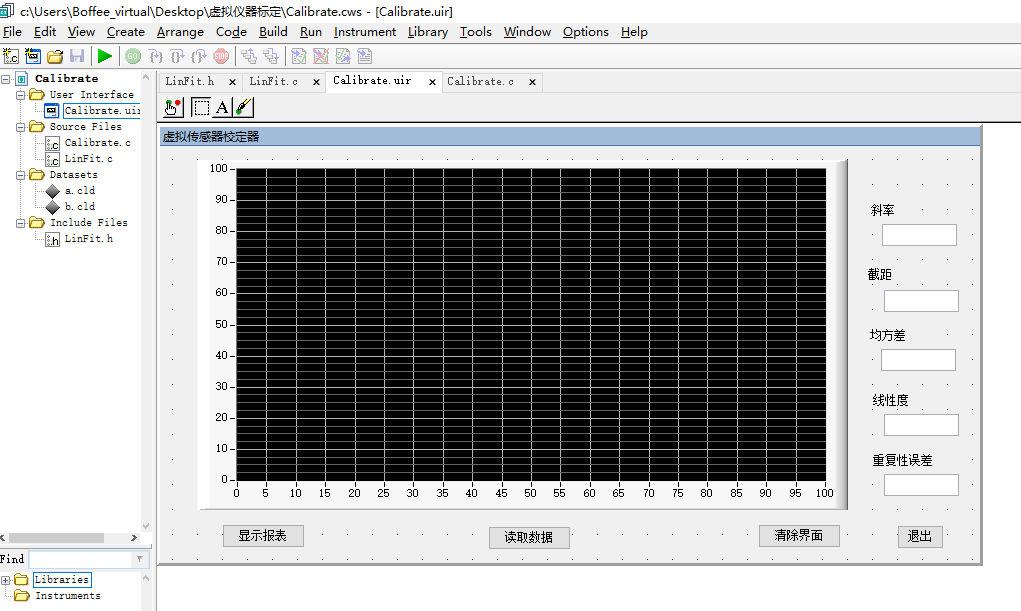
\includegraphics[width=0.8\textwidth]{图形用户界面设计示意图.png}
  \caption{图形用户界面设计示意图}
  \label{fig:ui}
\end{figure}
其中共有四个功能按键,分别为:
\begin{enumerate}
  \item 显示报表:将图形界面的数据以格式化文本形式输出至txt文件中;
  \item 读取数据:弹出文件选择对话框,选择数据文件,程序将自动实现解码与处理,并将结果可视化至坐标图中,将回归直线参数、线性度和重复性误差结果显示至右侧输出框中;
  \item 清除界面:清除坐标图和输出框,将缓冲区的数据清空;
  \item 退出:关闭程序。
\end{enumerate}
\section{实验结果}

\section{结论}

%% ----------- 附录部分 ------------ %%
\appendix
\appendixpage
\addappheadtotoc
\subappendix{ADT源代码}
这里是源代码
\subappendix{数据处理模块源代码}


\newpage
\printbibliography[heading=bibliography,title=参考文献]
\end{document}
